\PassOptionsToPackage{hyphens}{url}
\documentclass[11pt]{article}
\usepackage[margin=1in]{geometry}
\usepackage[T1]{fontenc}
\usepackage[utf8]{inputenc}
\usepackage{lmodern}
\usepackage{microtype}
\usepackage{amsmath,amssymb}
\usepackage{booktabs}
\usepackage{graphicx}
\usepackage{xcolor}
\usepackage{hyperref}

\hypersetup{
  colorlinks=true,
  linkcolor=blue!50!black,
  citecolor=blue!50!black,
  urlcolor=blue!50!black
}
\setlength{\emergencystretch}{2em}

\title{A Source-Frozen Multi-Readout Tau-Web Witness Protocol}
\author{J\'ozsef Olcs\'ak\\
\small Tau Core Research}
\date{November 14, 2026}

\begin{document}
\maketitle

\begin{abstract}
We present a source-frozen, reproducible multi-readout protocol (built from the
\texttt{TAU\_CORE\_FULL\_PACKAGE\_001} provenance suite) for evaluating
cosmic-web anisotropy candidates within the Tau Core empirical test program.
The central methodological rule is that single-channel galaxy filamentarity is
insufficient to define a Tau-compatible signal. Promotion to a witness
candidate requires survival across a predeclared multi-readout ladder:
systematics-cleaned galaxy and gravitational-lensing web tensors must align in
principal direction, the alignment must remain stable across redshift or radial
slices, declared survey-systematics projections must not absorb the signal,
source-native mock realizations must render the amplitude rare, and the
strongest witness class requires directional coherence with an independent third
tracer (such as peculiar velocities or CMB lensing). In the included
deterministic smoke benchmark, the pipeline executes every module and returns
\texttt{STRONG-WITNESS-CANDIDATE} (score $9.0$). Because the benchmark uses
synthetic smoke inputs rather than survey-grade maps and mocks, this outcome is
strictly an architectural and reproducibility verification: it is not a
real-data discovery, not a cosmological validation, and not a proof of Tau Core.
\end{abstract}

\section{Scope and Claim Boundary}

Paper 14 is a protocol paper.  It does not claim that Tau Core has detected a
cosmic-web residual, explained dark matter, replaced $\Lambda$CDM, or validated
a new gravitational theory.  Its purpose is narrower: to make explicit the
minimum source-frozen promotion rule by which a galaxy-side web anomaly could
become a Tau-compatible multi-readout witness candidate.

Terminology follows the current Tau Core convention.  A Tau-compatible web
witness would point, at most, to a web-scale \emph{morphological body}
\(M_\tau^\star\) (denoted \(M_\tau\) in legacy package headers) whose different
projected readouts include galaxy, lensing, velocity, or CMB-like web tensors.
The tensors scored here are downstream observational handles on that body, not
a direct reconstruction of it.

The input package is preserved in this repository as provenance.  The stable
smoke run is useful because it exercises the full protocol stack, not because
it is a survey endpoint.  Future validation requires real survey inputs,
source-native mocks, explicit covariance treatment, source-side freeze
artifacts, and blind endpoint scoring.  The natural survey context for such a
later test includes galaxy redshift surveys such as DESI \cite{desi2016},
CMB/lensing products such as Planck \cite{planck2018parameters}, and
independent lensing maps such as ACT DR6 \cite{actdr6lensing}.

Multi-readout alignment or covariance does not by itself identify a common
smooth parent transport. It is compatible with a common cause, overlapping
terminal information, or correlated nuisance structure. Under the current
Tau Core source boundary, a physical non-scalar transport must be supplied
independently as full body-connection holonomy or as Kato transport of a
varying source-owned access projector. The witness ladder below therefore
tests terminal coherence only; it does not reconstruct either source route.

\section{Tau-Web Witness Rule and Tensor Notation}

The starting rule is deliberately strict:
\[
\text{galaxy-only filamentarity} \neq
\text{Tau-compatible signal}.
\]
In Tau Core language, a candidate readout residual should not be promoted when
it appears in only one ordinary observational channel.  The minimum candidate
requires a cleaned galaxy web tensor and a cleaned lensing web tensor that
select the same tensor direction:
\[
W^{\mathrm{clean}}_{\mathrm{gal},ab} \parallel W^{\mathrm{clean}}_{\mathrm{lens},ab}.
\]

\paragraph{Notation disambiguation.}
Here $W^{\mathrm{clean}}_{\mathrm{gal},ab}$ and
$W^{\mathrm{clean}}_{\mathrm{lens},ab}$ denote symmetric, trace-free cosmic-web
anisotropy (tidal/morphology readout) tensors with spatial or sky-projected
indices $a,b$, obtained after projecting raw channel web tensors
$W^{\mathrm{raw}}_{c,ab}$ ($c \in \{\mathrm{gal},\mathrm{lens}\}$) orthogonal to
the predeclared survey-systematics subspace $\mathcal{S}_{\mathrm{sys}}$.
Repeated indices $a,b$ are contracted with the Euclidean frame metric so that
$\|W^{\mathrm{clean}}_c\| \equiv (W^{\mathrm{clean}}_{c,ab}
W_c^{\mathrm{clean},ab})^{1/2}$ is the Frobenius norm, and $W_{1,ab} \parallel
W_{2,ab}$ denotes unit-normalized tensor alignment up to positive scale.  To
prevent cross-paper symbol collisions, we emphasize that the tensor readout
symbol $W_{c,ab}$ in Paper~14 is unrelated to Paper~5's scalar phenomenological
finite-memory background kernel $W(x) = 1 + \rho x^3$ and distinct from the
canonical upstream dilogarithmic director-action density $W_{\mathrm{COCA}}(s)$
of the foundational seed--body kernel.

Operationally, the package evaluates the Frobenius tensor cosine
\[
C_{\mathrm{gal\text{-}lens}} =
\frac{W^{\mathrm{clean}}_{\mathrm{gal},ab} W_{\mathrm{lens}}^{\mathrm{clean},ab}}
{\left\|W^{\mathrm{clean}}_{\mathrm{gal}}\right\|
 \left\|W^{\mathrm{clean}}_{\mathrm{lens}}\right\|},
\]
the principal-axis alignment, redshift or radial slice stability, systematics
survival, and mock rarity.  A stronger witness candidate requires directional
coherence with an independent third readout,
\[
W^{\mathrm{clean}}_{\mathrm{gal},ab}
\parallel W^{\mathrm{clean}}_{\mathrm{lens},ab}
\parallel W^{\mathrm{extra}}_{ab}.
\]
In the included package the extra readout is represented by a velocity-channel
smoke component; the CMB-$\kappa$ extra readout remains absent in that run.

\begin{figure}[t]
\centering
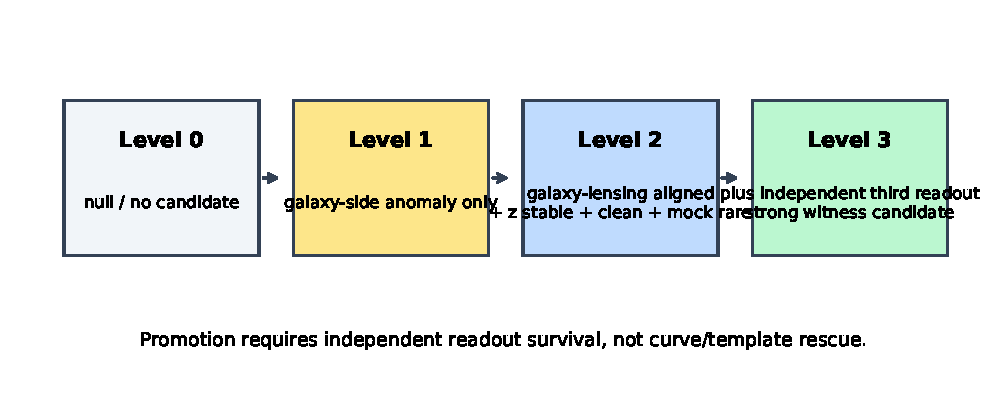
\includegraphics[width=0.95\linewidth]{figures/fig_tau_web_protocol_ladder.pdf}
\caption{Tau-web promotion ladder.  Galaxy-only filamentarity is retained as a
weak anomaly, not as a Tau-compatible candidate.  Promotion requires
cross-readout alignment, stability, systematics survival, mock rarity, and, for
the strongest candidate class, an independent third readout.}
\label{fig:ladder}
\end{figure}

\section{Pipeline Modules}

The protocol stack in \texttt{TAU\_CORE\_FULL\_PACKAGE\_001} separates the
following modules.

\begin{enumerate}
\item \textbf{Observation/readout tensor module.}  Build web tensors for galaxy
and lensing-like channels and compare their tensor directions.
\item \textbf{Redshift or radial stability module.}  Split the catalog into
slices and test whether the tensor direction remains stable.
\item \textbf{Weighted stability diagnostic.}  Allow a transparent weighted
rescue only when low-amplitude bins are the limiting factor.
\item \textbf{Systematics projector.}  Remove or project known systematics
directions and measure retained signal fraction.
\item \textbf{Mock covariance module.}  Compare the cleaned observed tensor to
mock realizations.
\item \textbf{Extra-readout module.}  Test whether a third independent channel
aligns with the same tensor direction.
\item \textbf{Verdict engine.}  Combine the above into an explicitly bounded
candidate status.
\end{enumerate}

This structure is intentionally leak-resistant: a candidate is not promoted by
choosing a better-fitting web template after seeing the endpoint residual.
Instead, each readout channel and threshold is declared before the verdict
engine is run.

\section{Stable Smoke-Run Summary}

The stable smoke run included in the package returns the verdict
\texttt{STRONG-WITNESS-CANDIDATE}.  Table~\ref{tab:summary} lists the main
quantities extracted by the reproduction script.

\begin{table}[htbp]
\centering
\begin{tabular}{lll}
\toprule
Quantity & Value & Module verdict\\
\midrule
$A_{\mathrm{gal}}$ & 0.6487 & \texttt{TAU-COMPATIBLE}\\
$A_{\mathrm{lens}}$ & 0.6466 & \texttt{TAU-COMPATIBLE}\\
$C_{\mathrm{gal\text{-}lens}}$ & 0.9999 & \texttt{TAU-COMPATIBLE}\\
axis alignment & 1.0000 & \texttt{TAU-COMPATIBLE}\\
$S_z^{\mathrm{tensor}}$ & 0.9590 & \texttt{Z-STABLE}\\
$S_z^{\mathrm{axis}}$ & 0.9901 & \texttt{Z-STABLE}\\
systematics retained fraction & 0.9066 & \texttt{CLEAN-CANDIDATE}\\
mock amplitude $p_{\mathrm{greater}}$ & 0.0123 & \texttt{MOCK-RARE-WEAK}\\
$C_{\mathrm{gal\text{-}velocity}}$ & 0.9999 & extra readout pass\\
final score & 9.0 & \texttt{STRONG-WITNESS-CANDIDATE}\\
\bottomrule
\end{tabular}
\caption{Stable smoke-run quantities.  These are protocol smoke-run outputs,
not validation-grade physical measurements.}
\label{tab:summary}
\end{table}

\begin{figure}[t]
\centering
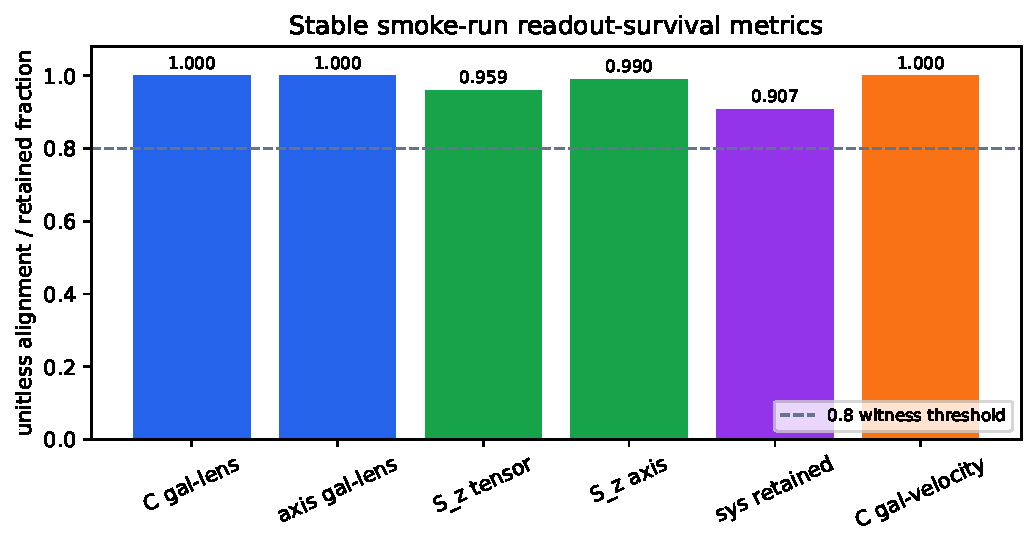
\includegraphics[width=0.92\linewidth]{figures/fig_tau_web_smoke_metrics.pdf}
\caption{Readout-survival metrics in the stable smoke run.  The dashed line is
the package's 0.8 reference threshold for alignment/stability quantities.}
\label{fig:metrics}
\end{figure}

\begin{figure}[t]
\centering
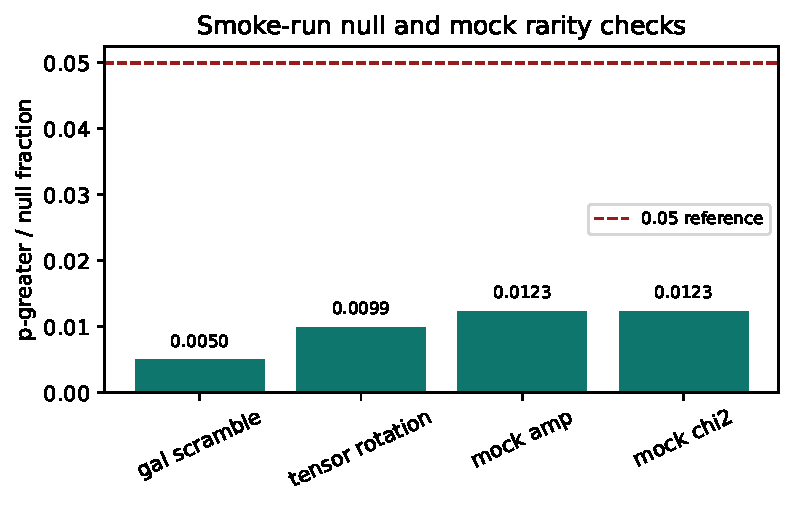
\includegraphics[width=0.72\linewidth]{figures/fig_tau_web_null_checks.pdf}
\caption{Null and mock rarity checks in the stable smoke run.  Values are
package-level $p_{\mathrm{greater}}$ or null fractions.  They are not discovery
$p$-values because the run is a protocol smoke test, not a real-survey endpoint.}
\label{fig:nulls}
\end{figure}

\section{Interpretation}

The smoke run demonstrates that the package can execute the intended finite
logic:
\[
D_{\mathrm{gal}}+D_{\mathrm{lens}}+D_{\mathrm{sys}}+D_{\mathrm{mock}}+D_z+D_{\mathrm{extra}}
\longrightarrow \text{bounded verdict}.
\]
The important theoretical gain is architectural.  Tau-compatible web evidence
is not allowed to mean ``a visually interesting galaxy distribution.''  It
means a cross-readout tensor relation that remains after stability, systematics,
mock, and optional third-readout checks.

This is a meaningful strengthening of the Tau Core architecture because it
turns the general multi-readout principle into a reproducible cosmic-web
protocol.  It also prevents overclaiming: a galaxy-only anomaly is explicitly
kept below the Tau-compatible candidate threshold.

A companion readout-covariance classifier protocol, Paper~17 in the Tau Core
sequence \cite{taucore2026paper17}, sharpens this interpretation.  It separates
shared-parent covariance support, denoted \(Z_{\mathrm{shared}}\), from
morphology or orientation support, denoted \(Z_{\mathrm{orient}}\).  Under that
stricter reporting rule, a visually convincing galaxy/lensing web alignment
would remain only an orientation-like candidate unless the shared-parent
covariance axis also survives.  Thus Paper~14's web-tensor alignment is a
candidate gate, not evidence by itself.

A companion photon-lensing Morphological Alignment Residual (MAR) protocol,
Paper~18 \cite{taucore2026paper18}, provides one concrete source-side
lensing/morphology statistic for this guarded ladder:
\(T_{\tau}=B_{\mathrm{env}}A_fM_{bf}\), where the angular mismatch term compares
baryon and filament orientation proxies.  Its v2 extension adds
out-of-sample scale validation, physical shear mocks, and a toy Null--Matter
Link diagnostic.  Those protocols are useful because they turn possible
web/lensing residuals into non-circular source-frozen templates, but they do
not promote the present smoke result.  MAR-type correlations remain
morphology/orientation support until a shared-parent covariance route survives
the Paper~17 controls \cite{taucore2026paper17}.

\section{Future Real-Data Endpoint}

A validation-grade version must replace the smoke package with source-native
survey products.  The expected first endpoint requires:

\begin{enumerate}
\item a DESI/LSS-like galaxy web readout with frozen footprint and mask rules;
\item a Planck, ACT, Euclid, Rubin, or equivalent lensing/mass-map readout;
\item source-native mocks and covariance;
\item blind source-side channel definitions;
\item explicit systematics projectors;
\item redshift-bin stability and weighted-stability rules declared in advance;
\item an independent third readout, such as velocity, CMB-lensing, ISW, or
another source-native tracer.
\end{enumerate}

The real-data endpoint should also be upgraded to the same v1.1 audit standard
used for the broader Tau Core reproducibility program:

\begin{enumerate}
\item \textbf{Raw-generator replay.}  Any mock or synthetic web/lensing source
block must be replayable from its seed, parent generator, feature matrix,
mask/selection rule, noise model, covariance rule, and train/held-out split.
\item \textbf{Sensitivity sweep.}  Candidate status must be checked against
predeclared variations of thresholds, ridge \(\lambda\) where a linear surrogate
is used, SNR or map-noise assumptions, feature dimensions, redshift-bin choices,
and held-out split definitions.
\item \textbf{Mock-catalog injection.}  Source-native mocks should inject known
web-aligned, misaligned, and systematics-dominated components before any
real-survey candidate is promoted.  This is the first serious bridge from a
smoke protocol to a realistic cosmic-web test.
\item \textbf{Independent implementation.}  A separate implementation should
rebuild the same frozen protocol and verify that the galaxy/lensing/extra-readout
pattern is reproduced without sharing the original analysis code.
\end{enumerate}

Until those conditions are met, the correct status is:
\[
\texttt{STRONG\_WITNESS\_CANDIDATE\_SMOKE\_ONLY}.
\]

\section{Full-4D Scoring Boundary}

The web-witness statistic is a protocol-specific morphology audit, not the
physical fixed Tau score.  The latter requires one source-frozen standard
excess
\[
 E_K=(K_{HH}-K_{\mathrm{std}})-CK_{VV}^{-1}C^\dagger
\]
and a common coframe push $E_g$, from which every jointly scored web,
lensing, velocity, or CMB terminal is generated.  Exact terminal duplicates
must be quotiented, but the remaining cross-terminal covariance must be kept.
Because this paper does not reconstruct such a nonzero $E_g$, its witness
scores are unchanged and cannot be read as a Tau-over-standard likelihood.

\section{Upstream Interface and Canonical Three-Pillar Bridge}
\label{sec:upstream-three-pillar-bridge}

% BEGIN OBSERVER UPDATE 20260914
\subsection{Observer Realization: Inherited Results and Physical Boundary}
\label{sec:observer-update-20260914}
The current observer programme distinguishes a conditional mathematical
construction from an occupied physical measuring system. The source order
remains base plus one universal seed, stabilized morphological response,
observer--source restriction, shared descriptor, and resolved terminal
readouts. Neither a detector nor an empirical residual constructs the parent
body backwards. Dynamics below concern downstream subsystems only.

Technical Paper TD-II (\emph{Body-to-Readout Derivation}) owns the following
results. The existing joint source action fixes static and frequency-dependent
response together. Variation of the BRAC potential couples to the field
square; a linear field coupling is a distinct comparator unless derived by
expansion about an occupied background. Fixed canonical means select a unique
coherent state in a finite positive harmonic packet only if there is no excess
fluctuation energy. This is a free/asymptotic preparation statement, not the
ground state of an interacting detector. For the existing coupled harmonic
pair, the joint ground is pure but either local subsystem is mixed, with its
covariance fixed by the complete joint Hamiltonian.

These are conditional derivations and internal numerical checks. The actual
observer--source context, physical preparation process, kinetic/energy
calibration and stable operational resolution remain unproved. The existing
ORA-T1 selector conditionally chooses stable quantizers when the occupied
context, admissible partition family and positive closure barrier are supplied;
it does not establish those physical premises. A computed ground state is not
a preparation mechanism, and a covariance or optimal abstract measurement is
not an implemented stable quantizer $Q_{OS}$.

\paragraph{Ownership and use.}
Technical Paper TD-II (\emph{Body-to-Readout Derivation}) carries the
consolidated contact, state, and covariance mathematics; Foundation Papers IV,
V, and VI retain physical-selection, clock-descent, and quantum-readout
ownership, respectively. This paper imports only the consequences within its
scope. No observational dataset, baseline, frozen coefficient, score, or
empirical conclusion is revised by this update.

\paragraph{Consequence for this paper.}
Different terminal labels are not independent information sources without a
factorization or novelty proof. A nonzero correlation is not automatically a
standard-orthogonal Tau signal.
% END OBSERVER UPDATE 20260914

% BEGIN STATE UPDATE 20260918
\subsection{Source Identification and Terminal Access}
The current observer audit separates a conditional forward construction from
physical source selection. A frozen body, occupied observer incidence,
preparation, complete instrument, and stable resolution can determine records
without selecting those inputs from Nature. Equal effects do not fix
postmeasurement states, and symmetry within a chosen interaction family does
not exclude other symmetric couplings. Different terminal labels are not
independent information sources without a factorization or novelty proof. A
nonzero correlation is not automatically a standard-orthogonal Tau signal.

\paragraph{Dependency and claim ownership.}
Foundation VI and Technical Paper TD-II own the finite instrument/access proof;
Foundation IV and TD-0 retain physical source selection; Foundation V, the
temporal synthesis, and the seed--body companion (TD-I) own the
gradient/inertial distinction. This paper inherits only the stated
specialization; canonical assumptions, countermodels, and calibration audits are
recorded in
\url{https://github.com/tau-core-research/tau-core-theory/blob/main/docs/tau_rqm_instrument_to_record_bridge_001.md}.
No physical seed, Nature occupation, or Tau-exclusive observation is established
by this update, and existing empirical endpoint definitions and scores are
unchanged.
% END STATE UPDATE 20260918

% BEGIN PAIR READOUT UPDATE 20260927
\paragraph{Imported result (CPR1).}
\href{https://github.com/tau-core-research/tau-core-higgs-module-paper4/blob/main/paper4_full_derivation/full_derivation.pdf#nameddest=cpr1}{Paper 4, \emph{Full Derivation Ledger for the Branch A Higgs Module}}, section ``Conditional source preparation and time-resolved access, Theorem CPR1(b,c),'' v1.0 (2026-09-28), is the sole proof owner.
Access-specific null directions must not be identified with nulls of the complete channel. The imported finite-sector example does not establish independent terminal information, photon or lensing recovery, or a Tau-specific correlation; empirical endpoints remain unchanged.
Physical preparation, detector/clock calibration and stable $Q_{OS}$ remain assumptions; no Tau-exclusive observation follows.
% END PAIR READOUT UPDATE 20260927

\subsection{Canonical Three-Pillar Reduction (2026-11-14)}
In the 2026-11-14 canonical reduction of the upstream Tau Core architecture
(Theorems U1--U4, F1--F4, \texttt{COV-DIR}, and \texttt{HOMOG-K4}), the minimal
symmetric $K_4$/Clifford algebraic lock fixes the seed projector ratio
$r_{\mathrm{seed}} = 1/4$ and the galactic readout slope
$\alpha_{\mathrm{OCSR}} = \frac{5\sqrt{3}}{24} \approx 0.360844$ with $k = 0$
adjustable continuous parameters, isolating a single remaining ontic physical
occupation postulate (\texttt{POST-OCC-NU1} / \texttt{EAS-SNPR-N1}). Within
this hierarchy, Paper~14's multi-readout web-tensor witness protocol evaluates
only downstream terminal alignment and mock-rarity gates on $W^{\mathrm{clean}}_{c,ab}$;
smoke-run verdicts remain methodological benchmarks rather than evidence for
physical occupation.

\section{Conclusion}

Paper 14 records a source-frozen multi-readout Tau-web witness protocol and a
complete stable smoke-run reproduction package.  The core claim is procedural:
galaxy-only filamentarity is insufficient, while a Tau-compatible cosmic-web
candidate must survive galaxy-lensing alignment, redshift stability,
systematics projection, mock rarity, and, for the strongest class, an
independent third readout.  The included smoke run exercises this full ladder
and reaches a strong candidate status inside the package grammar.  It does not
establish a real-data detection, cosmological validation, or physical proof of
Tau Core.

\bibliographystyle{plain}
\bibliography{refs}

\end{document}
